% !TeX root = ../FinalRepordCS.tex

\chapter{Implementation and Preliminary Performance Analysis}

\section{Implementation}
In this section, the primary emphasis is on executing the functionalities of LoRa nodes Alice and Bob by leveraging the Arduino programmable MCU board and IDE previously discussed. This implementation is conducted in tandem with the LoRa frequency modulation chip and the algorithms outlined earlier.

\begin{figure}
  \centering
  \subcaptionbox{LoRa Node Implementation\label{LoraNodeImplate}}
  {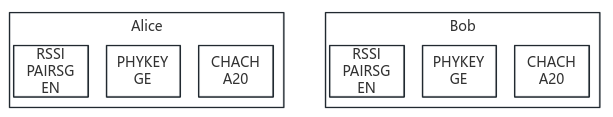
\includegraphics[width=0.8\linewidth]{LoraImplate.png}}
  \subcaptionbox{LoRa Transmission Implementation\label{LoraTransimissionImplate}}
  {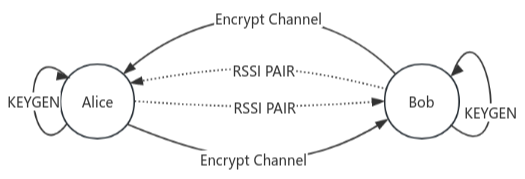
\includegraphics[width=0.7\linewidth]{LORAtransmit.png}}
  \caption{Implementation Details}\label{Implementation Details}
\end{figure}

As illustrated in Fiugre 5.1, The LoRa nodes mainly implemented the functions: 
\begin{itemize}
  \item RSSI key pairs generation 
  \item Physical layer bit code generation
  \item Chacha20 encrypt and decrypt
\end{itemize}

Also, the transmission protocol for physical layer key and encrypt communication channel has been implemented.
\begin{itemize}
  \item Half-duplex based RSSI pairs exchange protocol  
  \item Chacha20-based transmission for LoRa Protocol
\end{itemize}


\section{Deep-in-Building and Outdoor Test}
And after the implementation of the LoRa nodes, a practical test was undertaken to generate LoRa physical layer keys within a real-world application scenario including Deep-in-Building and Outdoor Test. The test yielded numerous results, thereby showcasing the tangible application of LoRa in real-world scenarios. Furthermore, the findings carry substantial reference value for informing and guiding the future deployment of the LoRa protocol, particularly in the context of environmental monitoring.

\subsection{RSSI Pairs Generation}

\begin{figure}
  \centering
  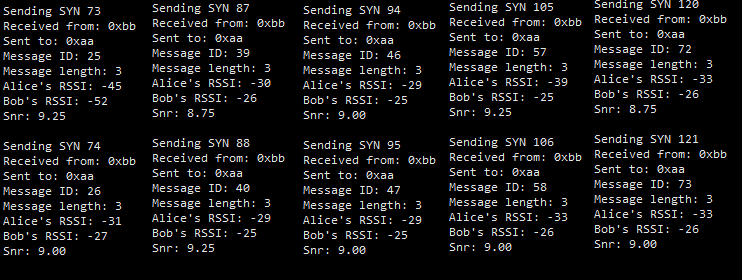
\includegraphics[width=0.9\linewidth]{fig5-1.png}
  \caption{Sampling in LoRa Node}
  \label{fig:5-1}
\end{figure}

\subsection{Key Generation}
Than a Python Program that implemented constitutes a crucial section of the thesis, focusing on LoRa physical layer key generation. Beginning with the processing of Received Signal Strength Indication (RSSI) data for both Alice and Bob, the code subsequently employs linear interpolation and Savitzky-Golay filtering to enhance the quality of the data.

Following these preprocessing steps, the script employs $M\--ary$ quantization on the smoothed RSSI values, utilizing a specified number of bits per sample and an alpha parameter. The homotopy method for error correction is then implemented, where a matrix \(A\) and vector \(y\) undergo iterative updates to correct errors in the data.

The key generation process involves the random generation of a matrix \(A\), the computation of vectors \(y_1\) and \(y_2\) based on the quantized data from Alice and Bob, and the application of error correction through the homotopy method. The final step involves XORing the original bits with the corrected bits to derive the cryptographic key.

The code also incorporates visualizations using Matplotlib to illustrate the impact of linear interpolation and Savitzky-Golay filtering on the original RSSI values. Additionally, the thesis section concludes with the presentation of crucial output information, including filtered RSSI arrays for Alice and Bob, and the original and corrected keys for Alice.
\begin{figure}
  \centering
  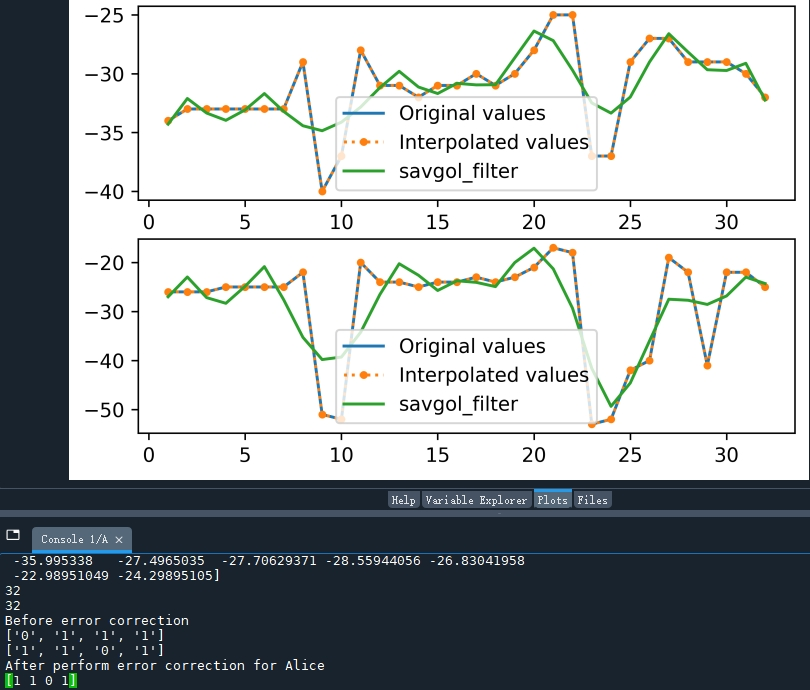
\includegraphics[width=0.9\linewidth]{fig5-2.png}
  \caption{Result of Performing Key Generation}
  \label{fig:5-2}
\end{figure}

\subsection{Data Encrypt and Decrypt}
Once the key has been generated, it can be employed alongside encryption algorithms to secure the data for transmission.

\begin{figure}
  \centering
  \subcaptionbox{Alice\label{Alice}}
  {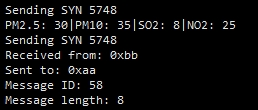
\includegraphics[width=0.4\linewidth]{chachaalice.png}}
  \subcaptionbox{Bob\label{Bob}}
  {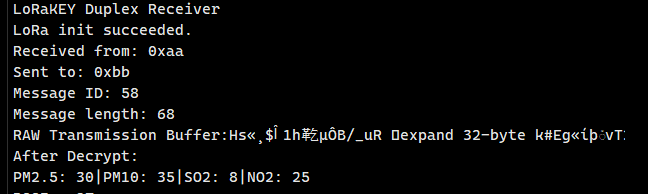
\includegraphics[width=0.7\linewidth]{chachabob.png}}
  \caption{Data Encrypt and Decrypt between Alice and Bob}\label{Data Encrypt and Decrypt}
\end{figure}

\section{Performance Analysis}
In this section, performance tests on password generation were implemented based on references, exploring the impact of different parameters. Additionally, the results were visualized for better comprehension of the test data.
